\chapter{Processes and protocols}
\section{Initialization of communication}
In order to establish a connection between the transmitter and receiver, these two devices must register with each other. Since the IoT transmitter is a device with very limited functions, it cannot register the receiver by input. Each transmitter is therefore equipped with a QR code. This QR code contains the address that can be used to communicate with the transmitter via Freenet.
The receiver registers the transmitter via its QR code. The address of the recipient is then transmitted to the sender via Freenet. The sender registers the recipient's address.
As soon as both sides have registered each other's communication path, an EC is sent to the receiver.
an ECDH (Elliptic Curve Diffie Hellman) is performed by both sides using the SecP256 elliptic curve. 
For this, an ECC (elliptic curve cryptography) key pair is created by both sides. 
The public key of the key pair is then forwarded to the other side via Freenet. Both sides calculate a shared secret after receiving the public key from the other side. Up to this point, the entire communication takes place on a non-secure channel. 
As soon as both parties have calculated the shared secret, both sides create new connection paths on Freenet. These paths are then encrypted with the shared secret and transferred to the other side.
Further communication then takes place via the secure channel created in this way.
\newpage
\subsection{SecP256r1 Elliptic curve}
SECP256r1 is an elliptic curve defined in SEC 2. It is an elliptic curve in the field \(z_p\), where \(p\) is a 256-bit prime. The "r" stands for random. The elliptic curve SECP256r1 has another sibling curve, the SECP256k1. The "k" stands for Koblitz. A Koblitz curve has some special properties that allow it to implement the group operations more efficiently. However, one assumes that a small security trade-off takes place, since often a greater "randomness" of the selected parameters leads to a higher security. For this reason, the elliptic curve SECP256r1 was used for the implementation of the prototype.
\begin{center}
\begin{figure}[!htb]
    \centering
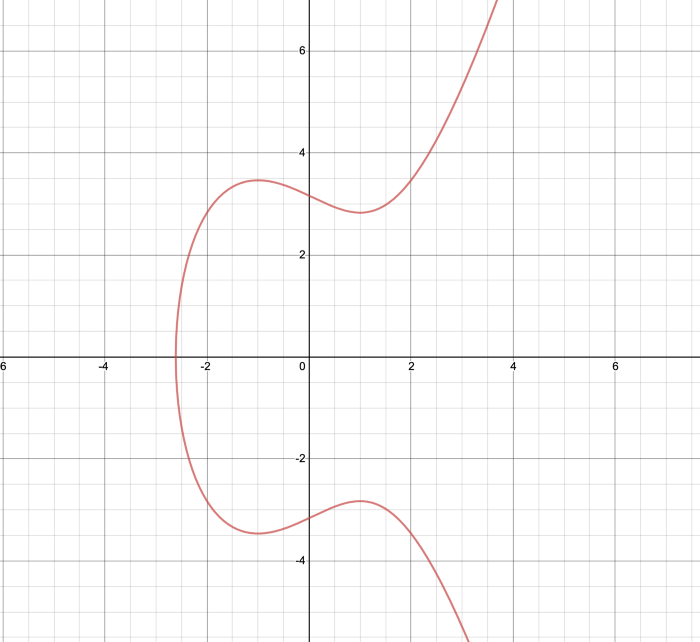
\includegraphics[width=6cm,height=8cm,keepaspectratio]{resources/images/NISTP256Curve.png}
    \caption{SecP256k1 Elliptic curve}
    \label{fig:DHKeyExchange}
\end{figure}
\end{center}
\newpage
\section{Initialization scheme}
\begin{center}
\rotatebox{90}{
\scalebox{0.7}{
\tcbox[top=0pt,left=0pt,right=0pt,bottom=0pt]{
\pseudocodeblock{
 \textbf{IoT sender} \< \< \textbf{Broker} \< \< \textbf{IoT receiver} \\[][\hline]
  \< \< \< \< \text{Register sender Freenet path } \\
  \< \< \< \sendmessageleft{top=Upload receiver Freenet path} \< \\
  \< \< \text{store receiver path} \< \< \\
  \< \sendmessageright{top=Get receiver path} \< \< \< \\
  \< \sendmessageleft{top=return receiver path} \< \< \< \\
  \text{Register receiver Freenet path} \< \< \< \< \\
\text{Gen random ECC key pair}  \< \< \< \< \text{Gen random ECC key pair} \\
 \< \sendmessageright{top=Upload sender pubkey} \< \< \sendmessageleft{top=upload receiver pubkey} \< \\
 \< \< \text{store information} \< \< \\
 \< \sendmessageleft{top=get receiver pubkey} \< \< \sendmessageright{top=get sender pubkey} \< \\
   \text{Calculate shared secret} \< \< \< \< \text{Calculate shared secret} \\
 \text{Gen new SSK Keypair} \< \< \< \< \text{Gen new SSK Keypair} \\
 \text{(Freenet path)} \< \< \< \< \text{(Freenet path)} \\
 \text{Encrypt Freenet path} \< \< \< \< \text{Encrypt Freenet path} \\
 \< \sendmessageright{top=Upload Freenet path} \< \< \sendmessageleft{top=Upload Freenet path} \< \\
 \< \< \text{store information} \< \< \\
 \< \sendmessageleft{top=get Freenet path} \< \< \sendmessageright{top=get Freenet path} \< \\
 \text{store receiver Freenet path} \< \< \< \< \text{store sender Freenet path} \\
}
}
}
}
\end{center}
